%% Преамбула TeX-файла

% 1. Стиль и язык
\documentclass[utf8x, 14pt]{G7-32} % Стиль (по умолчанию будет 14pt)

% Остальные стандартные настройки убраны в preamble.inc.tex.
\sloppy

% Настройки стиля ГОСТ 7-32
% Для начала определяем, хотим мы или нет, чтобы рисунки и таблицы нумеровались в пределах раздела, или нам нужна сквозная нумерация.
\EqInChapter % формулы будут нумероваться в пределах раздела
\TableInChapter % таблицы будут нумероваться в пределах раздела
\PicInChapter % рисунки будут нумероваться в пределах раздела

% Добавляем гипертекстовое оглавление в PDF
\usepackage[
bookmarks=true, colorlinks=true, unicode=true,
urlcolor=black,linkcolor=black, anchorcolor=black,
citecolor=black, menucolor=black, filecolor=black,
]{hyperref}

\AfterHyperrefFix

\usepackage{microtype}% полезный пакет для микротипографии, увы под xelatex мало чего умеет, но под pdflatex хорошо улучшает читаемость

% Тире могут быть невидимы в Adobe Reader
\ifInvisibleDashes
\MakeDashesBold
\fi

\usepackage{graphicx}   % Пакет для включения рисунков

% С такими оно полями оно работает по-умолчанию:
% \RequirePackage[left=20mm,right=10mm,top=20mm,bottom=20mm,headsep=0pt,includefoot]{geometry}
% Если вас тошнит от поля в 10мм --- увеличивайте до 20-ти, ну и про переплёт не забывайте:
\geometry{right=15mm}
\geometry{left=30mm}
\geometry{bottom=20mm}
\geometry{ignorefoot}% считать от нижней границы текста


% Пакет Tikz
\usepackage{tikz}
\usetikzlibrary{arrows,positioning,shadows}

% Произвольная нумерация списков.
\usepackage{enumerate}

% ячейки в несколько строчек
\usepackage{multirow}

% itemize внутри tabular
\usepackage{paralist,array}

%\setlength{\parskip}{1ex plus0.5ex minus0.5ex} % разрыв между абзацами
%\setlength{\parskip}{1ex} % разрыв между абзацами
\usepackage{blindtext}

% Центрирование подписей к плавающим окружениям
%\usepackage[justification=centering]{caption}

\usepackage{newfloat}
\DeclareFloatingEnvironment[
    placement={!ht},
    name=Equation
]{eqndescNoIndent}
\edef\fixEqndesc{\noexpand\setlength{\noexpand\parindent}{\the\parindent}\noexpand\setlength{\noexpand\parskip}{\the\parskip}}
\newenvironment{eqndesc}[1][!ht]{%
    \begin{eqndescNoIndent}[#1]%
\fixEqndesc%
}
{\end{eqndescNoIndent}}




% Настройки листингов.
\ifPDFTeX
% 8 Листинги

\usepackage{listings}

% Значения по умолчанию
\lstset{
  basicstyle= \footnotesize,
  breakatwhitespace=true,% разрыв строк только на whitespacce
  breaklines=true,       % переносить длинные строки
%   captionpos=b,          % подписи снизу -- вроде не надо
  inputencoding=koi8-r,
  numbers=left,          % нумерация слева
  numberstyle=\footnotesize,
  showspaces=false,      % показывать пробелы подчеркиваниями -- идиотизм 70-х годов
  showstringspaces=false,
  showtabs=false,        % и табы тоже
  stepnumber=1,
  tabsize=4,              % кому нужны табы по 8 символов?
  frame=single
}

% Стиль для псевдокода: строчки обычно короткие, поэтому размер шрифта побольше
\lstdefinestyle{pseudocode}{
  basicstyle=\small,
  keywordstyle=\color{black}\bfseries\underbar,
  language=Pseudocode,
  numberstyle=\footnotesize,
  commentstyle=\footnotesize\it
}

% Стиль для обычного кода: маленький шрифт
\lstdefinestyle{realcode}{
  basicstyle=\scriptsize,
  numberstyle=\footnotesize
}

% Стиль для коротких кусков обычного кода: средний шрифт
\lstdefinestyle{simplecode}{
  basicstyle=\footnotesize,
  numberstyle=\footnotesize
}

% Стиль для BNF
\lstdefinestyle{grammar}{
  basicstyle=\footnotesize,
  numberstyle=\footnotesize,
  stringstyle=\bfseries\ttfamily,
  language=BNF
}

% Определим свой язык для написания псевдокодов на основе Python
\lstdefinelanguage[]{Pseudocode}[]{Python}{
  morekeywords={each,empty,wait,do},% ключевые слова добавлять сюда
  morecomment=[s]{\{}{\}},% комменты {а-ля Pascal} смотрятся нагляднее
  literate=% а сюда добавлять операторы, которые хотите отображать как мат. символы
    {->}{\ensuremath{$\rightarrow$}~}2%
    {<-}{\ensuremath{$\leftarrow$}~}2%
    {:=}{\ensuremath{$\leftarrow$}~}2%
    {<--}{\ensuremath{$\Longleftarrow$}~}2%
}[keywords,comments]

% Свой язык для задания грамматик в BNF
\lstdefinelanguage[]{BNF}[]{}{
  morekeywords={},
  morecomment=[s]{@}{@},
  morestring=[b]",%
  literate=%
    {->}{\ensuremath{$\rightarrow$}~}2%
    {*}{\ensuremath{$^*$}~}2%
    {+}{\ensuremath{$^+$}~}2%
    {|}{\ensuremath{$|$}~}2%
}[keywords,comments,strings]

% Подписи к листингам на русском языке.
\renewcommand\lstlistingname{Листинг}
\renewcommand\lstlistlistingname{Листинги}

\else
\usepackage{local-minted}
\fi

% Полезные макросы листингов.
% Любимые команды
\newcommand{\Code}[1]{\textbf{#1}}


% Стиль титульного листа и заголовки
\gosttitle{Gost-report}       % Шаблон титульной страницы
% Варианты GostRV15-110 или Gost7-32 


%% Полное название организации
\ReportOrgLongName{Министерство образования и науки Российской Федерации}
%% Полное название университета
\ReportUniversity{Федеральное государственное автономное образовательное учреждение высшего образования \\ НАЦИОНАЛЬНЫЙ ИССЛЕДОВАТЕЛЬСКИЙ УНИВЕРСИТЕТ ИТМО}
%% Факультет
\ReportDepartment{Факультет Систем управления и Робототехники}
%% Дисциплина
\Report{<<Основы научно-технического творчества>>}
%% Тема
\ReportSubject{Ёмкостный датчик микроперемещений}
%% Вариант (если нет, то закомментируйте)
\ReportVariant{Патент № SU 1725070}


\ReportManager{Старший преподаватель}{Бушуев А.Б.} %% Преподаватель
\ReportIsp{R4135C}{Ураев И.С.} %% Студент

\ReportTown{Санкт-Петербург}

\begin{document}

\maketitle
\frontmatter % выключает нумерацию ВСЕГО
\tableofcontents % Содержание
\Introduction % Введение
\mainmatter % это включает нумерацию глав и секций в документе ниже
\bgroup
\titleformat{\chapter}
   {\normalfont\bfseries}{\hspace{12.5mm}\thechapter}{0.5em}{}
\titlespacing{\chapter}{0pt}{*4}{*1.5}

\titleformat{\section}
   {\normalfont\bfseries}{\hspace{12.5mm}\thesection}{0.5em}{}
\titlespacing{\section}{0pt}{*4}{*1.5}

%\titleformat{\section}
%   {\normalfont\bfseries}{\thesection}{1em}{}

\chapter{Описание прототипа}
%\label{cha:prorotype_description}
В описании авторского свидетельства № 1725070 МПК G01B 7/00 (по заявке № 4822394/28 от 22.03.90 г., автор В. Г. Панов) \cite{patent} представлено устройство «Ёмкосный датчик микроперемещений». Эскиз которого представлен на рисунке \ref{fig:draw}

\begin{figure}[]
    \centering
    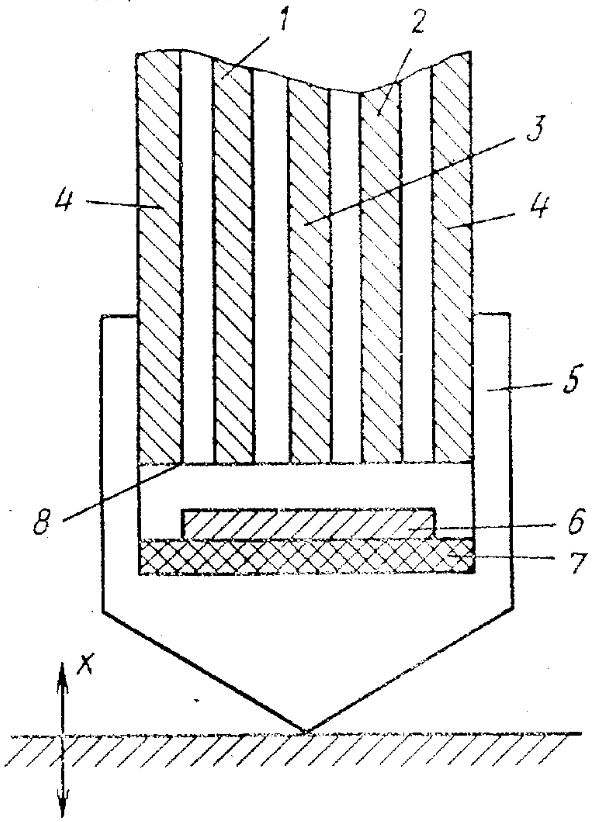
\includegraphics[width=0.7\textwidth]{graphics/img/draw.png}
    \caption{Эскиз прототипа}
    \label{fig:draw}
\end{figure}

Датчик содержит неподвижно закрепленные в корпусе потенциальный стержневой электрод 1 и установленный параллельно ему измерительный электрод 2, который отделен от потенциального электрода внутренним стержневым экраном 3. Внешний экран 4, выполненный в виде полого цилиндра, охватывает электроды датчика. Снаружи боковой цилиндрической поверхности внешнего экрана 4 размещен с возможностью возвратно-поступательного движения щуп 5, во внутренней полости которого размещена тонкая металлическая пластина 6, электрически изолированная от корпуса датчика с помощью диэлектрической прокладки 7 и расположенная параллельно рабочей плоскости 8 электродов и экранов датчика. Щуп 5 датчика упирается в поверхность контролируемого объекта, перемещение которого измеряется. 

Датчик работает следующим образом. При перемещении объекта изменяется воздушный зазор между плоскостью металлической пластинки 5 и рабочей плоскостью 8 электродов 1 и 2 и экранов 3 и 4 датчика, вследствие чего изменяется выходное напряжение $U_{\text{вых}}$ снимаемое с измерительного электрода 2 датчика. Чувствительность датчика зависит от величины диэлектрической постоянной материала контролируемого объекта и максимальна в диапазоне $[0 : x_{\text{мин}}]$, где $x$ - величина микроперемещения, когда металлическая пластина 6 не заземлена. Герметизация щупа 5 позволяет свести к минимуму погрешности, связанные с влиянием внешних условий.

\chapter{Анализ и синтез систем}
\label{cha:analis0}

\section{Анализ и синтез по закону полноты частей системы}

Полную ТС можно представить в виде структурной схемы, как показано на рисунке \ref{fig:analysis1_example}, где ЕЭ - источник энергии, а Изд. - изделие. Ро - рабочий орган, Тр - подводит энергию к Ро от Дв. (трансмиссия), Дв. - вырабатывает энергию, Оу - управляет работой всех или хотя бы одной частью системы. \cite{metodichka}

\begin{figure}
    \centering
    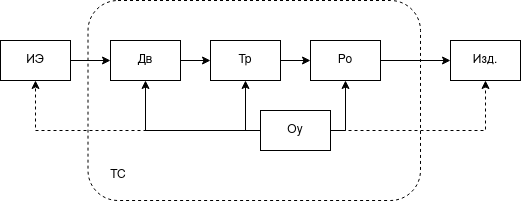
\includegraphics[width=0.8\textwidth]{graphics/img/analys1_example.png}
    \caption{Структурная схема полной технической системы}
    \label{fig:analysis1_example}
\end{figure}

Для описания по законы полноты частей системы следует определить основные функциональные элементы, представленные на рисунке \ref{fig:draw} соответствующие структурной схеме на рисунке \ref{fig:analysis1_example}.

Источником энергии в данной системе служит внешний источник питания, который подаёт питающее напряжение на потенциальный электрод и даёт ему положительный заряд.

Трансмиссией в данной системе служит потенциальный электрод 1. Преобразующий энергию в электромагнитное поле конденсатора между пластинами 1 и 6

Рабочим органом, органом управления, а также двигателем является щуп 5. Так как он непосредственно взаимодействует с измеряемой поверхностью перемещаясь перпендикулярно оси измеряемой плоскости. Щуп 5 приводится в движение за счёт давления оказанного от измеряемой плоскости. За счёт изменения воздушного зазора между электродами 1 и 6 изменяется и диэлектрическое сопротивление между ними, следовательно щуп 5 является и органом управления.

\section{Анализ и синтез по закону энергетической и информационной проводимости ТС}

Необходимым условием для принципиальной жизнеспособности ТС является сквозной проход энергии и информации по всем частям ТС. В соответствии с этим утверждением на рисунке \ref{fig:process} представлена линия прохода энергии/информации в анализируемой ТС.

\begin{figure}
    \centering
    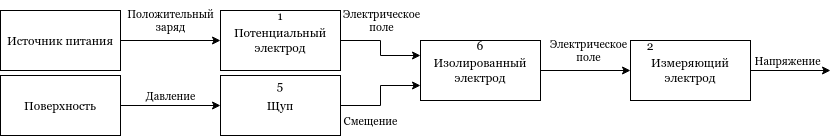
\includegraphics[width=\textwidth]{graphics/img/process_scheme.png}
    \caption{Линия прохода энергии/информации}
    \label{fig:process}
\end{figure}

Анализируя представленную схему можно заключить, что система разделяется на механическую (от поверхности производящее давление на щуп до измерительного электрода) и электрическую (от потенциального электрода, заряженного от внешнего источника питания к измерительному электроду) потоки энергии, где сводятся в один поток выдавая на выходе напряжение $U_{\text{вых}}$ соответствующая разности потенциалов между 1 и 2 электродами.

\section{Закон согласования-рассогласования технических систем}

 % Основная часть
\egroup
\backmatter % Убирает нумерацию снова
\Conclusion % Заключение
% % Список литературы при помощи BibTeX
% Юзать так:
%
% pdflatex rpz
% bibtex rpz
% pdflatex rpz

\bibliographystyle{ugost2008}
\bibliography{rpz}

%%% Local Variables: 
%%% mode: latex
%%% TeX-master: "rpz"
%%% End: 
 % Библиография

\end{document}


%%% Local Variables:
%%% mode: latex
%%% TeX-master: t
%%% End:
